%\documentclass{article} %[twocolumn] 
%\documentclass[Crown, times, sagev]{sagej}
\documentclass[sagev, Crown]{sagej} %

\usepackage{booktabs}
\usepackage{array}
\usepackage{graphicx}
\usepackage{amsmath}
\usepackage{amsfonts}
\usepackage{amssymb}
\usepackage{multirow}
\usepackage{url}

\setcounter{secnumdepth}{3} %Gives section numbers for cross referencing

% For submissing to Clinical trials: maximum 4,000 words excepting abstract, references, tables and figures; maximum 6 tables or figures.

\begin{document}

\runninghead{Wilson et al.}

\title{Three outcome designs for pilot trial progression criteria}

\author{Duncan T. Wilson\affilnum{1}}%,
%Rebecca E. A. Walwyn\affilnum{1}, 
%Julia Brown\affilnum{1} and 
%Amanda J. Farrin\affilnum{1}}

\affiliation{\affilnum{1}Leeds Institute of Clinical Trials Research, University of Leeds, Leeds, UK} %\\
%\affilnum{2}Centre for Primary Care \& Public Health, Queen Mary University of London, London, UK}

\corrauth{Duncan T. Wilson, Clinical Trials Research Unit, Leeds Institute of Clinical Trials Research, University of Leeds, Leeds, LS2 9JT, UK}
\email{d.t.wilson@leeds.ac.uk}

\begin{abstract}
The decision of if and how to progress to a definitive trial following a pilot study is often guided by progression criteria. Increasingly, progression criteria with three outcomes (stop, go, and an intermediate) are being used, but there is little methodological work examining how the thresholds or the pilot sample size should be determined. We review existing three-outcome designs and consider if and how they can be used to provide a formal statistical framework for pilot trials. We conclude that, contrary to previous claims, three-outcome designs do not improve efficiency, rather requiring a larger sample size than two-outcome alternatives. We also argue that pre-specified progression criteria are fundamentally ill-suited to pilot trials which lead to modifications of the trial design or the intervention before the main trial.
\end{abstract}

\keywords{Clinical trial, pilot trial, external pilot, progression criteria, sample size}

\maketitle

\section{Introduction}\label{sec:introduction}

When there is some uncertainty about the feasibility of a planned randomised clinical trial (RCT), a small version of the trial, known as an external pilot, can be conducted. The pilot data can be used to estimate various parameters of interest, such as the follow-up rate, and these estimates can then be used to decide if and how to proceed to the main trial. Investing in a pilot trial can identify potential issues at an early stage, make a successful main trial more likely, and reduce research waste.

The CONSORT extension to randomised pilot trials notes that progression decisions can be guided by so-called \emph{progression criteria} \cite{Eldridge2016a}. A simple progression criteria will prescribe a single threshold value, such that we should progress to the main trial only if the pilot estimate exceeds the threshold. When progression criteria are specified for several parameters, as is typically the case \cite{}, these can be combined by progressing to the main trial only if all of the estimates exceed their respective thresholds. In the UK, the NIHR requires that all pilot trials to have these progression criteria pre-specified at the design stage \cite{}.

Increasingly, more complex `traffic light' progression criteria are being used. These stipulate two threshold values for a given parameter of interest. If the estimate falls below the lower of these, the decision is to stop; if the estimate falls above the higher threshold, the decision is to proceed immediately to the main trial; and if the estimate falls between the two thresholds, an intermediate decision is reached. 

Three motivations for using a three-outcome system in pilot trials can be found in the literature. Firstly, it has been argued that making strict stop/go decisions based on a single threshold  may lead to the wrong decision by chance alone: ``\emph{estimates of rates in pilot trials may be subject to considerable uncertainty, so that it is best to be cautious about setting definitive thresholds that could be missed simply due to chance variation. In fact it is becoming increasingly common for investigators to use a traffic light system for criteria used to judge feasibility}'' \cite{Eldridge2016a}. By allowing for a buffer zone in between the `stop' and `go' regions, the probability of landing in these critical areas, and therefore of making incorrect decisions, will be reduced.

%This argument is paralled in the three outcome literaure, which argue that the designs can improve efficiency and either increase power, or reduce the required sample size.

A second motivation is to allow other information to inform the progression decision in the event of a `borderline' result. This might be attractive in the context of a pilot trial, where several aspects (quantitative and qualitative) are often being studied and we would like to be able to take these results into account rather than everything being decided on the result of a handful of estimates and their thresholds. Moreover, it could be argued this is how decisions are typically made even when a usual two-outcome system is nominally used.

A final reason for an intermediate outcome is to provide the flexibility needed to make some adjustment to the intervention or trial design in an attempt to improve the parameter in question and ensure the feasibility of the main trial. For example, after observing a mediocre follow-up rate in a pilot trial, we might consider moving from a postal follow-up strategy to one based on contacting the participants over the phone. This is perhaps the most prevalent reasoning given for three outcomes in pilot trials, with the intermediate `amber' decision often explicitly referred to as `amend' or `adjust' (examples).

Although prevalent, there is little methodological guidance to help researchers decide what threshold values to use in their progression criteria. The related question of pilot trial sample size is also methodologically undeveloped, with work in this area almost exclusively focussing on pilots whose primary function is to estimate the primary outcome variance to inform the main trial sample size calculation. These methods nevertheless are used when this is not the primary aim of the pilot, often in the form of simple `rules-of-thumb' \cite{Browne1995} \cite{Teare2014} \cite{Whitehead2015}. There are a number of papers, however, which propose designs for trials with three outcomes. Although typically proposed for phase II trials of cancer treatments, these three-outcome designs were motivated by the same factors given above, and so may provide a useful framework for the pilot trial setting.

In this paper we consider if, and how, three-outcome designs can be used to determine optimal pilot progression criteria and sample size. We begin in Section \ref{sec:tests} by arguing that progression criteria are mathematically equivalent to hypothesis tests and best viewed as such. In Section \ref{sec:review} we review three-outcome trial designs. We examine their statistical properties as applied to the progression criteria problem, and consider whether or not they can help with any of the three motivating goals (addressing sampling variability, incorporating other information, or allowing for adjustments), in Section \ref{sec:methods}. We illustrate our arguments via an example in Section \ref{sec:illustrate}, before concluding with a discussion in Section \ref{sec:discussion}.

\section{Progression criteria as hypothesis tests}\label{sec:tests}

Throughout this article we will focus on the simple case of a single parameter being assessed in the pilot trial: the adherence rate in the intervention arm. This will be sufficient to motivate and illustrate all our arguments. In particular, consider a two-outcome `stop/go' progression criterion for the adherence rate in the intervention arm of a pilot trial. Denoting the true (but unknown) adherence rate by $\rho$, the number of participants who adhere in the pilot trial will follow a binomial distribution with parameters $\rho$ and the intervention-arm sample size, denoted $n$. This data is then used to calculate the estimated adherence rate, denoted $\hat{\rho}$.

One way to make a stop/go decision based on $\hat{\rho}$ is through a hypothesis test, which can be constructed as follows. First, we identify a parameter value $\rho_0$ such that if $\rho \leq \rho_0$ we would like to limit the probability of incorrectly making a `go' decision (a type I error) to at most $\alpha$. Similarly, we identify $\rho_1$ such that if $\rho \geq \rho_1$ we would like to limit the probability of incorrectly making a `stop' decision (a type II error) to at most $\beta$. We denote by $x$ the critical value where if $\hat{rho} \geq x$ we reject the null hypothesis and make a `go' decision, otherwise choosing to `stop'. We then choose values of $n$ and $x$ which minimise $n$ whilst satisfying the type I and II error rate constraints
\begin{align}
\alpha = P[ \hat{\rho} > x ~ | ~ \rho = \rho_0] & \leq \alpha^* \\
\beta = P[ \hat{\rho} \leq x ~ | ~ \rho = \rho_1] & \leq \beta^*.
\end{align} 

Alternatively, we can work backwards and take any given choice for $n$ and $x$ and calculate the resulting error rates for some hypotheses $\rho_0, \rho_1$. In particular, whenever a pilot trial progression criteria is specified in the form of `if $\hat{\rho} \geq x$ then \emph{go} otherwise \emph{stop}', it is mathematically equivalent to a hypothesis test. For example, setting $n = 15$ and $x = 10/15$, we can plot the probability of making a `go' decision as a function of the unknown parameter $\rho$. This power curve is illustrated in Figure \ref{fig:power}.

\begin{figure}
\centering
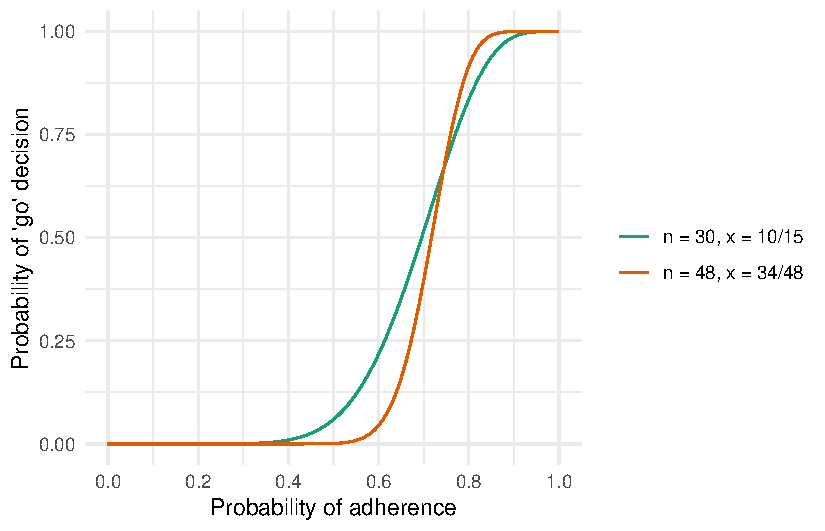
\includegraphics[scale=0.8]{./figures/power}
\caption{Power curves.}
\label{fig:power}
\end{figure}

If we suppose the null and alternatives hypotheses of interest are $\rho_0 = 0.6, \rho_1 = 0.8$ respectively, choosing $n = 15, x = 10/15$ gives error rates of $\alpha = 0.22$ and $1 - \beta = 0.84$. Alternatively, we can constrain the error rates to, for example, $\alpha^* = 0.05$ and $\beta^* = 0.1$, in which case the smallest possible sample size is $n = 48$ and the progression threshold is $x = 34/48$. The power curve for this design is plotted in Figure \ref{fig:power} for comparison. 

%It may be that $p$ is typically chosen to be the point such that, if $A = p$, we would be indifferent between stopping and going on to the main trial. This would effectively fix the power curve at 0.5 for $\rho = p/n$. The choice of $n$ will then determine power for the rest of the parameter space. It would appear that calculating this power explicitly, either for the whole parameter space of for the specific points $\rho_0$ and $\rho_1$, could only help find an appropriate value for $n$.

\section{Three-outcome clinical trial designs}\label{sec:review}

Multiple testing procedures for phase II trials, which we can think of as a three outcome design at each stage where the middle outcome is "go to next stage and test again". So, quite different to our problem because we want to change the intervention and then possibly start over again \cite{Fleming1982}. Similarly, \cite{Shuster2002} is just a two stage design, similar to \cite{Simon1989}. 

Motivated by the fact that we can't have both a low sample size and low alpha and betas. Suggests a three outcome model where the decisions are stop / slow development / accelerated development, allowing two extra types of errors to be allowed and controlled. Seems to be equivalent to a two-stage design since the middle outcome is to `do another study' \cite{Brown2012}, but maybe more pertinent to our external pilot situation.

Decision-theoretic (non-Bayesian) approach, giving different costs to different types of error. Motivated by contrasting one and two sided tests, looking for a method which can tell us if there is a significant direction in either direction or if there is no difference \cite{Emerson1987}.

A Class of Phase II Designs with Three Possible Outcomes \cite{Storer1992}. They propose an OC conditional on being in the middle of the parameter space, where ideally we want to make the intermediate decision.

A three-outcome design for randomized comparative phase {II} clinical trials \cite{Hong2007}. This just extends Sargent to a randomised case.

A review and comparison of early phase trial approaches \cite{Kirby2016}, including the three outcome design of \cite{Brown2012}.

Although far less prevalent than the standard two-outcome hypothesis test described in Section \ref{sec:tests}, various designs for trials with three outcomes have been proposed.

three outcome tests have been proposed. Following the same argument, we can show that a three-outcome progression criteria can be viewed as mathematically equivalent to a three-outcome design such as that described in \cite{Sargent2001}. This design specifies $n$ and two threshold, $p_0$ and $p_1$, and determines these based on four operating characteristics:
\begin{align}
P[ \hat{\rho} \geq p_1 | \rho = \rho_0] & = \alpha, \\
P[ \hat{\rho} < p_0 | \rho = \rho_1] & = \beta \\
P[ p_0 \leq \hat{\rho} < p_1 | \rho = \rho_0] & = \lambda \\
P[ p_0 \leq \hat{\rho} < p_1 | \rho = \rho_1] & = \delta.
\end{align}
By setting upper limits on $\alpha, \beta, \eta$ and $\pi$, we can identify the optimal trial design $n, p_0, p_1$.

\section{Three-outcome designs for progression criteria}\label{sec:methods}

As noted in Section \ref{sec:introduction}, there are three motivations for using three-outcome progression criteria. In this section we discuss if the three-outcome framework of Section \ref{sec:} can be used to address these goals.

\subsection{Addressing sampling variability}

use sargent here, since there and in extension they argue it reduces sample size.

For any given choice of nominal $\alpha$ and $\beta$, a three outcome design will have a lower required sample size providing the nominal $\lambda$ and/or $\delta$ are greater than 0. For example, take $\rho_0 = 0.5$ and $\rho_1 = 0.7$. A two outcome design will require $n = 53$ to ensure $\alpha \leq 0.05$ and $\beta \leq 0.1$. In contrast, by allowing $\lambda \leq 0.1$ and $\delta \leq 0.1$ in a three outcome design, we can obtain $\alpha \leq 0.05$ and $\beta \leq 0.1$ with only $n = 42$. This would suggest three outcome designs are indeed more efficient, as argued in \cite{Hong2007}. But this argument rests on a false equivalence, as we will show.

In \cite{Sargent2001} the authors state that ``We  can interpret $\alpha$  the usual  manner,  i.e., the  maximum probability of making an erroneous decision by rejecting the null hypothesis when in fact it is true''. To ``reject the null hypothesis'' here is to arrive at a `go' decision and proceed to the main trial. This decision, however, can be arrived at in two ways: directly, by obtaining $\hat{\rho} \geq p_1$; or indirectly, by first obtaining an intermediate result $p_0 \geq \hat{\rho} < p_1$ and then, after due consideration of whatever other information has been obtained in the pilot, deciding to proceed. Ultimately, we must always decide to either `stop' or 'go' to the main trial following an intermediate result in the pilot. Define
\begin{align}
\eta_0 &= P[\text{decide to `go'} | \rho = \rho_0, p_0 \geq \hat{\rho} < p_1] \\
\eta_1 &= P[\text{decide to `stop'} | \rho = \rho_1, p_0 \geq \hat{\rho} < p_1],
\end{align}
where e.g.  $\eta_0$ is the probability of making a 'go' decision following an intermediate result, when the true parameter value is $\rho_0$. The actual type I error rate, i.e. the probability of making a `go' decision when $\rho = \rho_0$, is
$$
\bar{\alpha} = \alpha + \eta_0 \lambda.
$$
Similarly, the actual type II error rate is
$$
\bar{\beta} = \beta + \eta_1 \delta.
$$
Under this reformulation of the three outcome design, we now estimate the probabilities $\eta_0, \eta_1$, set constraints on the actual type I and II error rates $\bar{\alpha}, \bar{\beta}$, and find the optimal design $n, p_0, p_1$. 

For simplicity we will assume that $\eta_0 = \eta_1 = \eta$; that is, the probability of eventually making the wrong decision following an intermediate result is the same for $\rho = \rho_0$ as for $\rho = \rho_1$. Returning to our example where $\rho_0 = 0.5, \rho_1 = 0.7, \bar{\alpha} \leq 0.05$ and $\bar{\beta} \leq 0.1$, we plot the required sample size for $0 \leq \eta \leq 0.5$ in Figure \ref{fig:}. 

We see that when $\eta = 0.5$, in which case we can only guess at the correct decision following an intermediate result, the optimal sample size is $n = 53$ and the three outcome design reduces to the two outcome design. At the other extreme, if $\eta = 1$ and we can decide without error, the tree outcome design reduces to a trivial one outcome design where an intermediate result is always obtained, upon which the correct stop/go decision can be reached. We see that for the kinds of sample size reductions given in \cite{Sargent2001}, we require $\eta$ of around 0.2. That is, we need to have an 80\% chance of correctly deciding to stop when we get an intermediate decision and the true parameter value is $\rho = \rho_0$; and similarly for deciding to proceed when $\rho = \rho_1$. In the context of our example, it is hard to think of a reason why our judgements would be so reliable. The appropriate default would seem to be $\eta = 0.5$. Unless we can argue that $\eta << 0.5$, the supposed efficiency of a three outcome design is an illusion, and its use will therefore not achieve the goal of better handling the sampling variability of parameter estimates in pilot trials.

\subsection{Incorporating other information}

use storer here

A corrolary of the above analysis is that when $\eta = 0.5$ the optimal deign is a two outcome design, with no amber region. If we want to have an amber region to provide opportunity to use other information in the case of a borderline result, we can go about this in a number of ways. 

We could decide on a fixed width, and then design to minimise $n$ s.t. the constraints as above.

We could allow the width to vary, but add another operating characteristic constraint, e.g. conditional on being midway between the null and alternative, we want a certain probability of making an amber decision. This is exaclty what was proposed in \cite{Storer1992}.

However we go about it, we know from the preceding section that to maintain the actual type I and II errors whilst introducing an amber region, we will have to \emph{increase} the sample size.

\subsection{Allowing for adjustments}

An alternative rationale for allowing three outcomes in a pilot trial is to enable some kind of adjustments to the trial design or intervention to be made upon obtaining a `borderline' result in the pilot. Under this setup, an intermediate result leads to an eventual `go' decision, but only after making some modification(s). Under the assumption that such modifications are always successful, the type I and II error rates are as above. 

We assume that a parameter in the amber region is salvageable, and will be salvaged if we get an amber decision. A red parameter is unsalvagable, regardless of the outcome. So, we could set up OCs: prob of infeasible trial = prob of a or g under R; prob of discarding intervention = prob of r under A or G, and of g under A; and prob of needless modification = prob of a under R or G. These are as in WP2. 

This only makes sense if we know what modifications will look like. In some cases this could feasibly apply. For example, we could consider improving recruitment by increasing the number of centres (although even here the size of the effect might be uncertain - see the Bayesian approach in \cite{Hampson2017}). But generally, the point of running the pilot is to identify issues which were not forseen. See the recruitment issue in \cite{Avery2017} - a staffing problem, which could be remidied and with a huge impact on recruitment rate, but where we would be guided into a stop decision becasue we did not allow for such a large modification effect. In the other direction, we might assume a large modification will be possible but not find any, landing us with a modify and go decision when we don't think this is sensible. In either case, we would ignore the pre-specified thresholds and use our judgement. But if this is the plan, why are we pre-specifying thresholds in the first place? If we are not certain about relying on our judgements, the best course of action may be to run another pilot with the changes made to check they are adequate. An adaptive design might make this process more efficient; or a factorial design trying lots of approaches at once and identifying the best to use in the main trial.

\section{Illustration}\label{sec:illustrate}

\section{Discussion}\label{sec:discussion}

We began by highlighting that pilot progression criteria are mathematically equivalent to a hypothesis test, but not designed with respect to the corresponding error rates. This might be a sensible reaction to the hegemony of this particular method, which has many shortcomings. Nevertheless, if we are working in a frequentist framework then the power curve as a function of $\rho$ and $n$ must be useful information, even if we use it more sensibly than via rigid type I and II error rate constraints. Note in particular that if progression criteria thresholds indicate the \emph{parameter} value which we would consider on the border of stop/go, then this will lead to a test with 50\% power at this inflection point - and it has been argued elsewhere that this is sensible. The choice of sample size can then be made conditional on this, using some other criteria, which could be power at a another specific point.

Pilot trial progression criteria are typically viewed as flexible guides to decision making, rather than cast-iron rules. This makes complete sense, and applies equally to the usual primary analysis tests where the p-value is not the last word in decision making. So, although we are not suggesting the rules are strictly followed, they can still be useful as a guide to decision making and choice of sample size.

An alternative approach to SSD is to focus on precision, rather than testing. But this appears to be much harder to reason about - how much precision do we want? Perhaps this is something which will emerge from experience?

Intermediate outcomes in pilots are never (?) used in an adaptive sense, i.e. where intermediate means collect more data. In contrast, this is the most common type of three outcome design in the drug trial literature, where many two-stage designs exist. An adaptive approach would help with objective 1 (efficiency), and could be used with a terminal intermediate outcome (in contrast to two stage designs which will have stop/go at the end to force a decision), using the above analysis to work out how much more sample size is needed to provide this flexibility. And indeed this aligns with \cite{Sargent2001}, who proposed one and two stage versions of their design. In the context of allowing modifications, we have the same problem of not being able to anticipate what they are or their effect. If we know what they are at least, an adaptive MAMS or factorial type approach evaluating several strategies and picking the winner - might be more efficient if data can be pulled for other parameters (e.g. if we have several recruitment strategies, but one follow-up, all arms can inform the follow-up estimate).


\begin{acks}
Acknowledgements.
\end{acks}

\begin{dci}
The Authors declare that there is no conflict of interest.
\end{dci}

\begin{funding}
This work was supported by the Medical Research Council [grant number MR/N015444/1].
\end{funding}

\bibliographystyle{SageV}
\bibliography{C:/Users/meddwilb/Documents/Literature/Databases/DTWrefs}

\section*{Appendix}


\end{document}